\documentclass[11pt]{article}
\usepackage[margin=1in]{geometry}
\usepackage{amsmath}
\usepackage{amssymb}
\usepackage{booktabs}
\usepackage{enumitem}
\usepackage{float}
\usepackage{graphicx}
\usepackage{tikz}
\usetikzlibrary{arrows.meta, positioning}

\title{Lecture Notes}
\author{CS186 - Database Systems}
\date{}

\begin{document}

\maketitle

\section{DBMS Architecture}

A user writes a SQL query, and somehow the right data comes back. In between, the DBMS handles several layers of work:

\begin{enumerate}
    \item \textbf{Parsing:} Check that the query is valid---tables and columns exist, syntax is correct.
    \item \textbf{Query planning and optimization:} Find an efficient way to execute the query (covered in later lectures).
    \item \textbf{Execution:} Run the plan, which ultimately requires reading data from disk.
    \item \textbf{File and disk management:} Decide which files to open, which pages to read, and how to transfer data between disk and memory.
\end{enumerate}

Each layer is an \textbf{abstraction} that hides the complexity beneath it. The user sees a flat relation with rows and columns. Underneath, the data may live in heap files, spread across disk pages, organized in packed or slotted layouts---none of which the user needs to know. This is \textbf{physical data independence}.

This lecture focuses on the bottom layers: how the DBMS stores data on disk and organizes it within files and pages.
\section{Storage Management}

A key design decision: \textbf{the data base management system does not rely on the OS file system for page management.}

The OS treats the DBMS as just another application. It doesn't know the query workload, so it can't make smart decisions like prefetching pages for a \texttt{SELECT *} scan. Instead, the DBMS asks the OS for one large file and manages pages within it internally. This lets the DBMS:

\begin{itemize}
    \item Control which pages are read and when.
    \item Prefetch pages when the query makes future reads predictable (e.g., a full table scan on a table spanning 10 blocks means we know we need all 10).
    \item Exploit knowledge of access patterns---for example, if a concert ticket table is being hit heavily, prefetch its blocks in advance.
\end{itemize}

For this course, assume \textbf{one file per relation} on a single disk.
\section{Disk I/O and Prefetching}

Since disk access is expensive, we want to \textbf{amortize} the cost by doing as much useful work per access as possible:

\begin{itemize}
    \item If pages for a table are stored \textbf{sequentially on disk}, we can read them in one sweep rather than jumping the disk arm around. This is much cheaper than scattered reads.
    \item If we can \textbf{predict future reads}, we can prefetch. Two sources of prediction:
    \begin{itemize}
        \item \textbf{The query itself:} \texttt{SELECT * FROM sailors} tells us we need every page of the sailors table.
        \item \textbf{Past access patterns:} If a table has been read frequently (e.g., during a ticket sale), it will likely be read again soon.
    \end{itemize}
\end{itemize}
\section{Heap Files}

A \textbf{heap file} is the simplest file structure: records are stored with no particular ordering. As tuples are inserted or deleted, pages are allocated or freed as needed.

To support basic operations (scan all records, insert, delete, retrieve by record ID), we need to track which pages exist and how much free space each has.

\subsection{Design 1: Linked List}

\begin{figure}[H]
    \centering  \includegraphics[width=0.8\textwidth]{images/heap_linkedlist.png}
    \caption{Heap file organized as a doubly linked list}
    \label{fig:heap_linkedlist}
\end{figure}

\begin{itemize}
    \item A \textbf{header page} points to two doubly linked lists: one of \textbf{full pages} and one of \textbf{pages with free space}.
    \item Each page stores a pointer to the next page and the previous page.
\end{itemize}

\textbf{Problem:} To insert a record, we need a page with enough free space. We may have to walk many links in the free-space list before finding one that fits (e.g., for a 20-byte record, many free pages might not have 20 bytes left). Retrieval of a specific record by ID also requires walking through pages sequentially.

\subsection{Design 2: Page Directory}

\begin{itemize}
\begin{figure}[H]
    \centering  \includegraphics[width=0.4\textwidth]{images/heap_directory.png}
    \caption{Heap file organized using a directory}
    \label{fig:heap_map}
\end{figure}
    \item A \textbf{directory} stores, for each page, a pointer to the page and the amount of free space it has.
    \item To insert, look up the directory for a page with sufficient space and jump directly to it---no linked list traversal.
    \item The directory can itself span multiple pages (a ``directory of directories'') if needed, though too many layers hit diminishing returns.
\end{itemize}

\textbf{Improvement over linked list:} Insertion is faster because we can locate a suitable page in one lookup instead of walking a chain. Full pages still appear in the directory (with free space recorded as zero).
\section{Page Layout}

Each page has a \textbf{header} with metadata: number of records, free space available, and pointers to other pages (if using the linked list design). The rest of the page holds records.

Two key design dimensions: Is the record size \textbf{fixed or variable}? And do we keep the page \textbf{packed or unpacked}?

\newpage
\subsection{Fixed-Length Records, Packed}

Records are stored contiguously, one after another, with no gaps.

\begin{figure}[H]
    \centering    \includegraphics[width=0.5\linewidth]{images/packed_records.png}
    \caption{Records Packed}
    \label{fig:placeholder}
\end{figure}


\begin{itemize}
    \item \textbf{Record ID} = (page ID, slot number). Locating record $i$: offset $= \text{header size} + i \times \text{record size}$. Simple arithmetic.
    \item \textbf{Insert:} Append at the end of the occupied region.
    \item \textbf{Delete:} Remove the record, then shift all subsequent records up to fill the gap (\textbf{consolidation}).
    \item \textbf{Scan:} Read from start to end. No gaps to skip. Very efficient.
\end{itemize}

\textbf{Trade-off:} Scans are fast (no holes), but deletions are expensive (must shift records to stay packed). Good when full scans are common and deletions are rare.

\subsection{Fixed-Length Records, Unpacked (Bitmap)}

Records occupy fixed slots, but gaps are allowed.

\begin{figure}[H]
    \centering    \includegraphics[width=0.5\linewidth]{images/unpacked_records.png}
    \caption{Records Unpacked}
    \label{fig:placeholder}
\end{figure}


\begin{itemize}
    \item A \textbf{bitmap} in the page header tracks which slots are occupied (1) and which are empty (0).
    \item \textbf{Record ID} = (page ID, slot number). Locating a record still uses arithmetic, but we check the bitmap first.
    \item \textbf{Insert:} Find an empty slot via the bitmap, write the record, flip the bit.
    \item \textbf{Delete:} Flip the bit to 0. No consolidation needed.
    \item \textbf{Scan:} Must consult the bitmap to skip empty slots. Gaps may also cause non-sequential disk reads within the page.
\end{itemize}

\textbf{Trade-off:} Deletions are cheap (just flip a bit), but scans are slightly more complex and may encounter holes. Good when deletions are frequent and full scans are less critical.

\subsection{The Core Trade-off: Pack Now or Pay Later}

\begin{itemize}
    \item \textbf{Packed:} Pay at deletion time (consolidation) to keep things tidy. Scans are fast later.
    \item \textbf{Unpacked:} Pay at scan time (skipping holes, checking bitmaps). Deletions are fast now.
\end{itemize}

The right choice depends on whether 
there are frequent scans or frequent insertions and deletions.

\subsection{Variable-Length Records: Slotted Page}

When records have variable lengths, we cannot use simple arithmetic to locate records. Instead, we use a \textbf{slotted page} design.

\begin{figure}[H]
    \centering
    \includegraphics[width=0.6\linewidth]{images/slotted_page.png}
    \caption{Slotted Page Layout}
    \label{fig:slotted_page}
\end{figure}

\begin{itemize}
    \item A \textbf{slot directory} (also called the footer) stores metadata at one end of the page. Each slot entry contains a \textbf{pointer} to a record and optionally its length.
    \item \textbf{Records} are stored at the opposite end of the page and grow toward the middle.
    \item \textbf{Free space} sits between the slot directory and the records.
    \item \textbf{Record ID} = (page ID, slot number). External references use slot numbers, not physical offsets.
\end{itemize}

\subsubsection*{Why Grow in Opposite Directions?}

Since records are variable-length, we don't know how many will fit on a page. If the slot directory were at the top followed immediately by records, adding a new slot would require shifting all records which is expensive.

By having the slot directory grow upward and records grow downward (or vice versa), we avoid this problem:
\begin{itemize}
    \item \textbf{Insert:} Add a new slot entry (grows toward middle), write the record (grows from other end). No shifting required.
    \item \textbf{Page full:} When the two regions meet, allocate a new page.
\end{itemize}

\subsubsection*{Operations}

\begin{itemize}
    \item \textbf{Insert:} Find free space, write the record, add a slot entry pointing to it.
    \item \textbf{Delete:} Mark the slot as empty. This leaves a hole in the record area.
    \item \textbf{Compaction:} Periodically, the page can be \textbf{compacted}---records are moved to eliminate holes, and slot pointers are updated. Crucially, \textbf{slot numbers do not change}, so external references (from indexes or other pages) remain valid.
    \item \textbf{Scan:} Iterate through the slot directory, following each pointer to read records.
\end{itemize}

\subsubsection*{Trade-offs}

\begin{itemize}
    \item \textbf{Flexibility:} Handles variable-length records gracefully.
    \item \textbf{Stable references:} Slot numbers stay constant even when records move during compaction.
    \item \textbf{Overhead:} Requires storing a pointer (and possibly length) for every record, unlike fixed-length packed pages where position is implicit.
\end{itemize}

\textbf{Real-world usage:} PostgreSQL and MySQL both use slotted page designs. It is the standard approach for handling variable-length records in modern database systems.
\section{Cost Model}

To compare different file organizations, we need a quantitative way to measure performance. Unlike Big-O analysis, which ignores constant factors, \textbf{constant factors matter} in database systems.

\subsection{Why I/O Cost?}

Different hardware (spinning disks, SSDs) have different speeds, so wall-clock time is not a portable metric. Instead, we count \textbf{I/O operations}: the number of page reads and writes. This provides a hardware-independent basis for comparison.

To convert to actual time, multiply by a technology-specific factor $D$ (average time to read/write one page).

\subsection{Simplifying Assumptions}

For our analysis, we make several simplifications:

\begin{itemize}
    \item Ignore the difference between sequential and random reads.
    \item Ignore prefetching.
    \item \textbf{Ignore CPU cost} Only I/O operations count.
    \item Ignore metadata and header overhead.
    \item Data must be brought into memory before processing; writes must go back to disk. Both incur I/O cost.
\end{itemize}

\subsection{Operations of Interest}

We analyze five operations on two file types (heap file and sorted file):

\begin{enumerate}
    \item \textbf{Scan:} Read all records in the file.
    \item \textbf{Equality search:} Find a record with a specific key value.
    \item \textbf{Range search:} Find all records with keys in a given range.
    \item \textbf{Insert:} Add a new record.
    \item \textbf{Delete:} Remove a record.
\end{enumerate}


\subsection{Key Variables}

\begin{table}[H]
    \centering
    \begin{tabular}{cl}
        \toprule
        \textbf{Variable} & \textbf{Meaning} \\
        \midrule
        $B$ & Number of blocks (pages) \\
        $R$ & Average number of records per page \\
        $D$ & Time to read or write one block to disk\\
        \bottomrule
    \end{tabular}
    \caption{Cost model variables}
    \label{tab:cost_variables}
\end{table}

\subsection{Cost Summary}

\begin{table}[H]
    \centering
    \begin{tabular}{lcc}
        \toprule
        \textbf{Operation} & \textbf{Heap File} & \textbf{Sorted File} \\
        \midrule
        Scan all records & $B \cdot D$ & $B \cdot D$ \\
        Equality Search & $0.5 \cdot B \cdot D$ & $(\log_2 B) \cdot D$ \\
        Range Search & $B \cdot D$ & $((\log_2 B) + B) \cdot D$ \\
        Insert & $2 \cdot D$ & $((\log_2 B) + B) \cdot D$ \\
        Delete & $(0.5 \cdot B + 1) \cdot D$ & $((\log_2 B) + B) \cdot D$ \\
        \bottomrule
    \end{tabular}
    \caption{I/O cost comparison (average case)}
    \label{tab:cost_comparison}
\end{table}

\subsection{The Core Trade-off}

\begin{itemize}
    \item \textbf{Heap files} are fast for insertions (just append) but slow for searches (must scan).
    \item \textbf{Sorted files} are fast for searches (binary search) but slow for insertions and deletions (must maintain order).
\end{itemize}

The optimal choice depends on the workload:
\begin{itemize}
    \item Read-heavy $\rightarrow$ sorted file
    \item Write-heavy $\rightarrow$ heap file
\end{itemize}

Neither structure excels at both. This limitation motivates the need for \textbf{indexes}, which aim to provide fast searches without expensive insertions and deletions.
\section{Indexes}

From the previous lecture, we saw the fundamental trade-off between heap files and sorted files:

\begin{table}[H]
    \centering
    \begin{tabular}{lcc}
        \toprule
        \textbf{Operation} & \textbf{Heap File} & \textbf{Sorted File} \\
        \midrule
        Equality Search & $0.5 \cdot B \cdot D$ & $(\log_2 B) \cdot D$ \\
        Insert & $2 \cdot D$ & $((\log_2 B) + B) \cdot D$ \\
        \bottomrule
    \end{tabular}
    \caption{The core trade-off}
    \label{tab:tradeoff}
\end{table}

\begin{itemize}
    \item \textbf{Heap files:} Fast inserts (just append), slow searches (must scan).
    \item \textbf{Sorted files:} Fast searches (binary search), slow inserts (must shift records to maintain order).
\end{itemize}

\textbf{Goal:} Can we achieve fast searches \textit{without} expensive inserts? This motivates the need for indexes.

\subsection{What Is an Index?}

An index is a data structure that allows us to look up records using a \textbf{search key}, similar to the index at the back of a book.

\begin{itemize}
    \item The search key does not have to be the primary key.
    \item Can be built on any column(s) we frequently query.
    \item Can be non-unique (multiple records may share the same key).
\end{itemize}

\textbf{Example:} If queries frequently search by \texttt{student\_id}, build an index on that column. If queries search by \texttt{major}, build an index on \texttt{major} instead.
\section{B+ Trees}

\subsection{Sorted File with Holes}

Start with a heap file, sort it, but leave empty slots in each page.

\textbf{Why leave holes?}
\begin{itemize}
    \item Insertions and deletions no longer require shifting all records.
    \item New records can fill existing holes.
\end{itemize}

\textbf{Trade-off:} More pages are needed to store the same amount of data, since each page is partially empty.

\textbf{Remaining problem:} Binary search still has a fanout of 2 (we can only go left or right at each step). Can we do better?

\subsection{Separating Keys from Data}

Split storage into two types of pages:

\begin{figure}[H]
    \centering
    \includegraphics[width=0.8\linewidth]{images/key_datapage.png}
    \caption{Data pages store full records (tuples), while key lookup pages store only the indexed column value and a pointer to the record's location.}
    \label{fig:placeholder}
\end{figure}

\textbf{Why this helps:}
\begin{itemize}
    \item Keys are smaller than full tuples (one column vs.\ many columns).
    \item More keys fit per page $\rightarrow$ fewer pages to search through.
    \item Data pages no longer need to be sorted. The key pages handle navigation.
\end{itemize}

\textbf{What a key page entry stores:}
\begin{enumerate}
    \item The key value (e.g., \texttt{major} or \texttt{nameLast}).
    \item A pointer to where the record lives (page ID, slot ID).
\end{enumerate}

This is analogous to a book index. At the back of a textbook, you might find:

\begin{table}[H]
    \centering
    \begin{tabular}{ll}
        \toprule
        \textbf{Topic} & \textbf{Page} \\
        \midrule
        B+ trees & 142\\
        Binary search & 58 \\
        Hash tables & 97 \\
        \bottomrule
    \end{tabular}
\end{table}

\begin{itemize}
    \item \textbf{Key:} The topic name (``B+ trees'')
    \item \textbf{Pointers:} The page numbers (142)
\end{itemize}

You don't store the entire explanation of B+ trees in the index but rather just enough to tell you where to find it. Database indexes work the same way.

\subsection{Tree Structure}

Instead of binary search on key pages, build a tree structure with \textbf{high fanout}.

\begin{itemize}
    \item \textbf{Binary tree:} Fanout of 2 (go left or right).
    \item \textbf{B+ tree:} Fanout of hundreds or thousands (many children per node).
\end{itemize}

\begin{figure}[H]
    \centering
    \includegraphics[width=0.8\linewidth]{images/B+_tree.png}
    \caption{B+ Tree Structure}
    \label{fig:bplustree}
\end{figure}

\subsubsection*{Sorting Property}

Keys within each node are \textbf{sorted}. When searching for a key, you compare your search value against the keys to decide which pointer to follow.

\textbf{Example:} Searching for 27 in an interior node with keys [5 $|$ 13 $|$ 24]:
\begin{itemize}
    \item Values $\leq 5$: follow leftmost pointer
    \item Values $> 5$ and $\leq 13$: follow second pointer
    \item Values $> 13$ and $\leq 24$: follow third pointer
    \item Values $> 24$: follow rightmost pointer
\end{itemize}

Since $27 > 24$, we follow the rightmost pointer. This process repeats at each level until we reach a leaf.

\subsubsection*{Properties of B+ Trees}

\begin{itemize}
    \item \textbf{Balanced:} All leaf nodes are at the same depth/level, guaranteeing consistent search performance.
    \item \textbf{High fanout:} Each node contains many keys and pointers, reducing the number of levels needed.
    \item \textbf{Data at leaves only:} Interior nodes store keys and pointers to child pages; only leaf nodes store pointers to actual records.
    \item \textbf{Linked leaves:} Leaf pages are doubly linked, enabling efficient range scans (find keys $>= 27$) without traversing back up the tree.
    \item \textbf{Occupancy invariant:} Every node (except the root) must be at least half full. This helps the tree maintain a high fanout, and prevents it from degenerating into a binary tree.
\end{itemize}

\subsubsection*{Why High Fanout Matters}

With a binary tree (fanout 2), searching 1 million records requires $\log_2(1{,}000{,}000) \approx 20$ levels.

With a B+ tree (fanout 2,000), the same search requires $\log_{2000}(1{,}000{,}000) \approx 2$ levels.

Fewer levels means fewer page reads (each level is one page read), which means faster searches.

\textbf{Why high fanout matters:}

\begin{table}[H]
    \centering
    \begin{tabular}{lcc}
        \toprule
        \textbf{Tree Type} & \textbf{Fanout} & \textbf{Height for 4 million records} \\
        \midrule
        Binary tree & 2 & $\approx 22$ levels \\
        B+ tree & 2,000 & 2 levels \\
        \bottomrule
    \end{tabular}
    \caption{Impact of fanout on tree height}
    \label{tab:fanout}
\end{table}

Disk reads are expensive because data must be loaded from disk into memory. Once data is in memory, we treat computation on it as free.

\textbf{Note:} We don't load all keys onto one page and do binary search because page size is fixed by the hardware. We can't create one giant page containing all the keys, and for large datasets (millions or billions of records), the keys wouldn't fit anyway.

\textbf{Note:} Disk I/O (reading/writing) is expensive because data must be transferred from disk into memory. Computation performed entirely in memory is treated as free.

\subsection{B+ Tree Insertion}

Insertion in a B+ tree always begins at the leaf level. When inserting a key into a B+ tree:
\begin{itemize}
    \item We search down the tree to find the correct leaf node.
    \item Insert the key in sorted order.
    \item If the leaf has room, we are done.
\end{itemize}
Most insertions are straightforward. We simply find the appropriate leaf and place the key in its sorted position. The tree structure only changes when a node overflows.

\textbf{Splitting a Leaf Node when it overflows:}

Each node has a maximum capacity. When a node becomes full and we attempt to insert another key, the node \textbf{overflows} and must be \textbf{split}.

\begin{figure}[H]
    \centering
    \includegraphics[width=0.5\linewidth]{images/leafInsertionex1.png}
    \caption{61 was attempted to be inserted, but the node was already at its maximum size of 4.}
    \label{fig:placeholder}
\end{figure}

Divide the keys: the smaller half go into the left node, the larger half go into the right node.

\begin{figure}[H]
    \centering
    \includegraphics[width=0.5\linewidth]{images/leafInsertionex2.png}
    \caption{61 was attempted to be inserted, but the node was already at its maximum capacity, triggering a split due to the max node size.}
    \label{fig:placeholder}
\end{figure}

Next, we copy up the middle key (smallest key of the right node or largest in the left node) into the parent as a separator.

\begin{figure}[H]
    \centering
    \includegraphics[width=0.5\linewidth]{images/leafInsertionex3.png}
    \caption{The middle key, 73, is copied up into the parent node to act as a separator between the left node (61, 67) and the right node (79, 97).}
    \label{fig:placeholder}
\end{figure}

The parent now points to both the left and right nodes, with the copied-up key acting as a \textbf{separator}, where all keys in the left subtree are less than or equal to it, and all keys in the right subtree are greater than it.

\textbf{Splitting an Interior Node:}
 
Divide the keys: the smallest half go into the left node, the largest half go into the right node.

\begin{figure}[H]
    \centering    \includegraphics[width=0.5\linewidth]{images/interiorInsertionex1.png}
    \caption{The full interior node is split: keys are divided so that 17 and 23 move into the left node, while 31 and 37 move into the right node.}
    \label{fig:placeholder}
\end{figure}

Redistribute the child pointers appropriately between the two new nodes.

\textbf{Push up} the middle key into the parent. If the parent is already full, it will overflow, and we repeat the splitting process on the parent with recursion.

\begin{figure}[H]
    \centering
    \includegraphics[width=0.5\linewidth]{images/interiorInsertionex2.png}
    \caption{Child pointers are redistributed to match the split, and the middle key, 43, is copied upward from the original node.}
    \label{fig:placeholder}
\end{figure}

\begin{figure}
    \centering
    \includegraphics[width=0.5\linewidth]{images/interiorInsertionex3.png}
    \caption{The middle key, 43, becomes the new parent node, with the left child containing keys 11 and 29 and the right child containing keys 67 and 89, completing the recursive split.}
    \label{fig:placeholder}
\end{figure}

Splitting is a \textbf{recursive} process. When we split a node and push a key into the parent, the parent may itself overflow. If so, we repeat the splitting process on the parent.

\textbf{Example:} Suppose we insert a key into a full leaf. We split the leaf and push a key into the parent. But the parent was already full, so it now overflows. We split the parent into two nodes and push a key into the grandparent. This process continues up the tree as needed.

\textbf{The tree node grows taller only when the root splits.} In this case:
\begin{itemize}
    \item Split the root into two nodes.
    \item Create a new root node containing the pushed-up middle key.
    \item The new root points to the two nodes created from the old root.
\end{itemize}

This ensures the tree remains \textbf{balanced}, where all leaves stay at the same depth. The tree grows from the root upward, not from the leaves downward.

\subsection{B+ Tree Deletion}

To delete a key, we search for it using the standard search algorithm, remove it from its node, and if the node still has at least the minimum number of keys, we are done.

However, sometimes when we delete a key, it causes a node to have fewer than the minimum number of keys. When this happens, we borrow a key from a node next to it/sibling.

\begin{figure}[H]
    \centering
    \includegraphics[width=0.5\linewidth]{images/underflowDeleteex1.png}
    \caption{Deleting key 16 causes the leaf node to underflow, leaving it with fewer than the minimum number of keys.}
    \label{fig:placeholder}
\end{figure}


When borrowing from the right sibling when it has more than the minimum number of keys, we take the smallest key from the right sibling, which becomes the new separator in the parent. The old separator from the parent moves down to fill the gap in the underflowing node.

\begin{figure}[H]
    \centering
    \includegraphics[width=0.5\linewidth]{images/underflowDeleteex2.png}
    \caption{The underflowing node borrows from its right sibling: key 21 becomes the new separator in the parent, and the old separator moves down to restore the minimum occupancy.}
    \label{fig:placeholder}
\end{figure}

If we instead borrow from the left sibling, we take the largest key from the left sibling, which becomes the new separator in the parent.

\textbf{Important:} We cannot simply move a key directly from sibling to sibling. The separator key in the parent must be updated to maintain the B+ tree property (all keys to the left of a separator are smaller; all keys to the right are larger).

If neither sibling can spare a key (both are at minimum occupancy), we must \textbf{merge} nodes. 

\begin{figure}[H]
    \centering
    \includegraphics[width=0.5\linewidth]{images/merge1.png}
    \caption{Neither sibling can spare a key, so the underflowing node and its sibling are selected for merging, along with the separator key from the parent.}
    \label{fig:placeholder}
\end{figure}

We do this by combining the node where a key was deleted, a sibling node, and the separator between them, and merging them into a single full node.

\begin{figure}[H]
    \centering
    \includegraphics[width=0.5\linewidth]{images/merge2.png}
    \caption{The nodes are merged into a single node containing keys 18, 20, 21, and 24, and the separator is removed from the parent.}
    \label{fig:placeholder}
\end{figure}

After merging, the parent may itself underflow. If so, we recursively apply the same strategy: first try to borrow from a sibling, and if that fails, merge with a sibling.

The tree becomes shorter when a merge propagates all the way to the root and the root ends up with no keys. In this case:
\begin{itemize}
    \item The root is deleted.
    \item The single remaining child of the old root becomes the new root.
\end{itemize}

This is the only way the tree's height decreases, maintaining the property that all leaves are at the same level.

\textbf{Deleting from Interior Nodes.}

When the key to be deleted is in an interior node (acting as a separator), we need a replacement separator.

\begin{figure}[H]
    \centering
    \includegraphics[width=0.5\linewidth]{images/interior1.png}
    \caption{Key 28 is deleted from an interior node, leaving a gap that requires choosing a replacement separator from one of its subtrees.}
    \label{fig:placeholder}
\end{figure}

A valid replacement must be:
\begin{itemize}
    \item Greater than all keys in the left subtree, and
    \item Smaller than all keys in the right subtree.
\end{itemize}

So we must choose either the \textbf{largest key in the left subtree} or the \textbf{smallest key in the right subtree.} We replace the deleted key with the chosen candidate, then delete the candidate from its original leaf node. 

\begin{figure}[H]
    \centering
    \includegraphics[width=0.5\linewidth]{images/interior2.png}
    \caption{The separator is replaced using the smallest key in the right subtree.}
    \label{fig:placeholder}
\end{figure}

This may trigger underflow handling in that leaf, but we just fix it buy borrowing a key from a sibling or merging with a sibling.

\subsection{Leaf Page Organization}

B+ tree leaf pages can be organized in different ways depending on how they connect to the actual data. This choice affects lookup speed, storage requirements, and how many indexes you can create.

We want multiple B+ trees because a single B+ tree can only speed up queries on the column(s) it's indexed on. For example, if you have a B+ tree on \texttt{player\_id}, a query like \texttt{WHERE name = 'Joe'} can't be used. You'd need a separate B+ tree on \texttt{name}. Since we often want multiple indexes (B+ trees) per table, the way we organize leaf pages matters.


\subsubsection*{Alternative 1: Storing By Value}
\begin{itemize}
    \item Store the actual tuples directly in the leaf pages
    \item One fewer pointer to follow allowing faster lookups
    \item Leaves become much larger since they hold full tuples, not just pointers
    \item You can only have ONE such index (B+ Tree) per table. If you want a second index, you have to duplicate your data.
\end{itemize}

\subsubsection*{Alternative 2: By Reference}
\begin{itemize}
    \item Leaf pages store pointers (page number + record ID) to tuples
    \item This is the standard approach we've been using
    \item Allows multiple indexes on the same table  (each index just stores pointers to the same data)
\end{itemize}

\subsubsection*{Alternative 3: List of References}
\begin{itemize}
    \item Like Alternative 2, but stores a \textit{list} of pointers per key
    \item Useful when multiple records share the same key (e.g., many players named ``Joe'')
    \item To find a specific record among duplicates, you have to follow each pointer and check one by one
\end{itemize}

\subsection{Clustered vs Unclustered}

Clustering refers to whether the data pages themselves are sorted by the index key. This affects how efficiently we can read data, especially for range queries.

\subsubsection*{Clustered Index}
\begin{itemize}
    \item The data pages are \textbf{sorted} by the index key (essentially a sorted file with a B+ tree on top)
    \item Pointers from leaf pages go in parallel, no criss-crossing
    \item \textbf{Pro:} Range queries are fast \texttt{(e.g., WHERE birth\_year > 1970}). Find the starting point and read sequentially 
    \item \textbf{Pro:} Nearby keys are stored on nearby (or the same) pages
    \item \textbf{Con:} Harder to maintain, as Insertions may require shuffling data to keep things sorted
    \item In practice, pages are kept about $\frac{2}{3}$ full to leave room for future inserts
\end{itemize}

\subsubsection*{Unclustered Index}
\begin{itemize}
    \item The data pages are a \textbf{heap} (unsorted)---the B+ tree is built on top of unordered data
    \item Pointers from leaf pages go everywhere
    \item \textbf{Pro:} Easier to maintain. Inserts just go wherever there's space
    \item \textbf{Con:} Range queries are slow. You may have to jump to many different pages
\end{itemize}

\subsubsection*{Why Only One Clustered Index Per Table?}

You can only sort your data \textbf{one way}. Think of it like arranging chairs in a room. You can sort them by age or by color, but not both at the same time unless you duplicate them.

Since a clustered index requires the data pages to be sorted by that index's key, you can only have \textbf{one clustered index per table}. Any additional indexes must be unclustered (they just point to wherever the data happens to be).

\subsubsection*{Sequential vs Random I/O}

This matters because of how disks work:
\begin{itemize}
    \item \textbf{Sequential reads} (clustered): Reading consecutive pages is fast; up to 100$\times$ faster on spinning disks
    \item \textbf{Random reads} (unclustered): Jumping around to different pages is slow, as the disk arm has to move each time
\end{itemize}

For SSDs, this difference is smaller, but sequential reads are still faster.

\subsection{Composite Indexes}

When you create a composite index on multiple columns, the order matters. The data is sorted by the first column, then by the second column as a tiebreaker, and so on.

Suppose we have a B+ tree index on \texttt{(birth\_year, weight)}. Which queries can use the index?

\begin{table}[H]
    \centering
    \begin{tabular}{lcp{7cm}}
        \toprule
        \textbf{Query} & \textbf{Can use index?} & \textbf{Why?} \\
        \midrule
        \texttt{birth\_year = 1970} & Yes & Directly matches the first indexed column \\
        \texttt{weight > 200} & No & Weight is only the tiebreaker. \\
        \texttt{birth\_year = 1970 AND weight > 200} & Yes & Find all 1970 records, then filter by weight (which is sorted within that group) \\
        \texttt{birth\_year > 1970} & Yes & Find the first 1970 record, then read everything to the right \\
        \bottomrule
    \end{tabular}
\end{table}

The first column in a composite index \texttt{(birth\_year, weight)} has more significance. You can only use the index efficiently if your query includes the first column. Queries on just the second column can't use the index.

\subsection{I/O Cost}

We want to compare B+ trees against heap files and sorted files. Remember: we count I/O operations (page reads/writes), not Big-O complexity. Constant factors matter in databases.

\subsubsection*{Key Variables}

\begin{table}[H]
    \centering
    \begin{tabular}{cl}
        \toprule
        \textbf{Variable} & \textbf{Meaning} \\
        \midrule
        $B$ & Number of data pages (if fully packed) \\
        $D$ & Time to read/write one page \\
        $R$ & Records per page \\
        $F$ & Fanout (typically $\approx 2000$, \textbf{not} 2) \\
        $E$ & Entries per leaf page \\
        \bottomrule
    \end{tabular}
\end{table}

\subsubsection*{Why Fanout Matters}

Both sorted files and B+ trees have logarithmic lookup time, but:
\begin{itemize}
    \item Sorted file (binary search): $\log_2(n)$
    \item B+ tree: $\log_F(n)$ where $F \approx 2000$
\end{itemize}

$\log_{2000}(n)$ is \textbf{much smaller} than $\log_2(n)$. For 1 million records:
\begin{itemize}
    \item Binary search: $\log_2(1{,}000{,}000) \approx 20$ page reads
    \item B+ tree: $\log_{2000}(1{,}000{,}000) \approx 2$ page reads
\end{itemize}

This is why B+ trees beat sorted files---same Big-O, but the constant factor is huge.

\subsubsection*{Cost Formulas}

\textbf{Scan all records:}
\[
\text{Cost} = 1.5 \cdot B \cdot D
\]
The $1.5$ factor comes from pages being $\frac{2}{3}$ full (we leave room for inserts). We don't need the index for this---just read all data pages.

\textbf{Equality search:}
\[
\text{Cost} = \left( \log_F \left( \frac{B \cdot R}{E} \right) + 2 \right) \cdot D
\]
\begin{itemize}
    \item $\log_F(\ldots)$: traverse the tree from root to leaf
    \item $+1$: accounts for reading the root
    \item $+1$: fetch the actual data page (following the pointer)
\end{itemize}

\textbf{Range search:}
\[
\text{Cost} = \left( \log_F \left( \frac{B \cdot R}{E} \right) + \text{num\_pages} \right) \cdot D
\]
Find the starting point, then read all matching pages. In a clustered index, these pages are sequential.

\subsubsection*{Cost Comparison}

\begin{table}[H]
    \centering
    \begin{tabular}{lccc}
        \toprule
        \textbf{Operation} & \textbf{Heap File} & \textbf{Sorted File} & \textbf{B+ Tree (Clustered)} \\
        \midrule
        Scan & $B$ & $B$ & $1.5B$ \\
        Equality Search & $0.5B$ & $\log_2 B$ & $\log_F B$ \\
        Range Search & $B$ & $\log_2 B + \text{pages}$ & $\log_F B + \text{pages}$ \\
        \bottomrule
    \end{tabular}
    \caption{I/O cost comparison (in page reads, $D$ omitted)}
\end{table}

\subsubsection*{Key Takeaways}

\begin{itemize}
    \item \textbf{Constant factors matter}: $\log_F$ vs $\log_2$ makes a big difference when $F \approx 2000$
    \item \textbf{Sequential I/O $\gg$ Random I/O}: on spinning disks, sequential reads are $\sim$100$\times$ faster
    \item \textbf{Clustered indexes} allow sequential reads for range queries; unclustered indexes require random reads
    \item The $1.5\times$ scan cost comes from leaving pages $\frac{2}{3}$ full for future inserts
\end{itemize}
\section{KD Trees}

B+ trees work well for one-dimensional data, but they struggle with multi-dimensional queries. Consider a B+ tree index on \texttt{(birth\_year, weight)}:

\begin{table}[H]
    \centering
    \begin{tabular}{lcp{7cm}}
        \toprule
        \textbf{Query} & \textbf{Can use index?} & \textbf{Why?} \\
        \midrule
        \texttt{birth\_year = 1970} & Yes & Matches the first indexed column \\
        \texttt{weight > 200} & No & Weight is only a tiebreaker; data isn't sorted by weight alone \\
        \texttt{birth\_year = 1970 AND weight > 200} & Yes & Filter by birth\_year first, then weight \\
        \bottomrule
    \end{tabular}
\end{table}

The problem: B+ trees impose an \textbf{ordering} on attributes. The first column dominates, and queries on only the second column cannot use the index.

\textbf{Real-world applications needing multi-dimensional queries:}
\begin{itemize}
    \item \textbf{Astronomy:} Find all stars within a region of the sky, or find the nearest star to a given point.
    \item \textbf{Video games:} Determine which objects appear on screen, or detect collisions between characters.
    \item \textbf{Databases:} Filter on multiple attributes without being forced into a specific order.
\end{itemize}

A \textbf{KD tree} (K-dimensional tree) is a binary tree that enables efficient queries across multiple dimensions. The key idea: instead of always splitting on the same attribute, we can split on \textbf{different dimensions} at each level.

\begin{itemize}
    \item \textbf{K} refers to the number of dimensions (e.g., 2D for x and y coordinates).
    \item Each internal node splits the space along one dimension.
    \item Each leaf node contains a single point (or a page of points in practice).
\end{itemize}

\textbf{Supported queries:}
\begin{itemize}
    \item \textbf{Point lookup:} Find a specific point by its coordinates.
    \item \textbf{Range search:} Find all points within a rectangular region.
    \item \textbf{Nearest neighbor:} Find the closest point to a given location.
\end{itemize}

\subsection{KD Tree Construction}

To build a KD tree, we recursively split the points in half until each region contains exactly one point.

\textbf{Algorithm:}
\begin{enumerate}
    \item \textbf{Base case:} If there is only one point, create a leaf node.
    \item \textbf{Otherwise:}
    \begin{itemize}
        \item Choose a dimension to split on (can alternate or choose strategically).
        \item Find the \textbf{median} value along that dimension.
        \item Split the points into two halves: those less than the median go left, those greater go right.
        \item Recursively build subtrees for each half.
    \end{itemize}
\end{enumerate}

\textbf{Why use the median?} The median guarantees an equal split of points, keeping the tree \textbf{balanced}. A balanced tree has fewer levels, which means fewer disk I/Os during queries.

\subsubsection*{Step-by-Step Example}

We will construct a 2D tree from 8 points: A, B, C, D, E, F, G, H.

\textbf{Step 1: First split on X-axis}

We start with all 8 points. Choose the X dimension and find the median X value, which we call $x_1$. This splits the points into two equal halves: 4 points on the left (A, B, C, D) and 4 points on the right (E, F, G, H).

\begin{figure}[H]
    \centering
    \includegraphics[width=0.8\textwidth]{images/kdtree1.png}
    \caption{Initial split on the X-axis at $x_1$. The tree now has a root node storing $x_1$.}
    \label{fig:kdtree1}
\end{figure}

\textbf{Step 2: Split the left half on Y-axis}

Now we focus on the left region (points A, B, C, D). We choose the Y dimension and find the median Y value, $y_1$. This splits the 4 points into: 2 points below $y_1$ (A, B) and 2 points above $y_1$ (C, D).

\begin{figure}[H]
    \centering
    \includegraphics[width=0.8\textwidth]{images/kdtree2.png}
    \caption{The left half is split on the Y-axis at $y_1$. The tree grows: $x_1$ points to $y_1$ as its left child.}
    \label{fig:kdtree2}
\end{figure}

\textbf{Step 3: Split the lower-left region on X-axis}

The lower-left region contains points A and B. We split on X again, using median value $x_2$. This separates A and B into their own leaf nodes.

\begin{figure}[H]
    \centering
    \includegraphics[width=0.8\textwidth]{images/kdtree3.png}
    \caption{The lower-left region is split at $x_2$, separating points A and B into individual leaves.}
    \label{fig:kdtree3}
\end{figure}

\textbf{Step 4: Split the upper-left region on Y-axis}

The upper-left region contains points C and D. We could split on X, but these points are stacked vertically, so splitting on Y (using $y_2$) creates more balanced regions. This separates C and D.

\begin{figure}[H]
    \centering
    \includegraphics[width=0.8\textwidth]{images/kdtree4.png}
    \caption{The upper-left region is split at $y_2$, separating points C and D. Note: we split on Y again, not X---this is allowed.}
    \label{fig:kdtree4}
\end{figure}

\textbf{Step 5: Split the right half on Y-axis}

Now we return to the right region (points E, F, G, H). We split on Y using median $y_3$, creating an upper-right region (G, H) and a lower-right region (E, F).

\begin{figure}[H]
    \centering
    \includegraphics[width=0.8\textwidth]{images/kdtree5.png}
    \caption{The right half is split on the Y-axis at $y_3$. The root's right child is now $y_3$.}
    \label{fig:kdtree5}
\end{figure}

\textbf{Step 6: Split the lower-right region on Y-axis}

The lower-right region contains points E and F. We split on Y using $y_4$ to separate them.

\begin{figure}[H]
    \centering
    \includegraphics[width=0.8\textwidth]{images/kdtree6.png}
    \caption{The lower-right region is split at $y_4$, separating points E and F.}
    \label{fig:kdtree6}
\end{figure}

\textbf{Step 7: Split the upper-right region on X-axis}

Finally, the upper-right region contains points G and H. We split on X using $x_3$ to separate them. The tree is now complete.

\begin{figure}[H]
    \centering
    \includegraphics[width=0.8\textwidth]{images/kdtree7.png}
    \caption{The upper-right region is split at $x_3$, separating points G and H. Construction is complete.}
    \label{fig:kdtree7}
\end{figure}

\textbf{Optional optimization:} Just like in B+ trees, the leaf nodes can be linked together with pointers, enabling efficient full scans without traversing the tree structure.

\subsubsection*{Key Observations}

\begin{itemize}
    \item \textbf{Dimensions can repeat:} We split on Y twice in a row (at $y_1$ and $y_2$) for the left side. There is no requirement to strictly alternate X, Y, X, Y.
    \item \textbf{Split values are independent:} $y_1$, $y_2$, $y_3$, and $y_4$ are all median of the points in that specific region.
    \item \textbf{The tree records the splitting history:} Each path from root to leaf encodes which regions a point belongs to.
    \item \textbf{Each node stores its split dimension:} We need to know whether a node splits on X or Y to perform queries correctly (typically stored as a bitmap).
\end{itemize}

\subsubsection*{Choosing the Split Dimension}

Two common strategies:

\begin{table}[H]
    \centering
    \begin{tabular}{lp{10cm}}
        \toprule
        \textbf{Strategy} & \textbf{Description} \\
        \midrule
        Round-robin & Alternate dimensions at each level: X, Y, X, Y, ... Simple to implement. \\
        Adaptive & Choose the dimension that creates the most ``square-like'' regions. Avoids long, thin rectangles that require more splits. \\
        \bottomrule
    \end{tabular}
\end{table}

\textbf{Why avoid thin rectangles?} If regions become long and skinny, you need more splits to separate points, leading to a deeper tree and more I/O operations during queries.

Just like with heap files, sorted files, and B+ trees, we analyze KD trees by counting \textbf{I/O operations} (page reads/writes), not Big-O complexity. Constant factors matter in database systems.


\subsection{Point Lookup}

To find a specific point, we traverse from the root to a leaf, comparing against the split dimension at each level.

\[
\text{Cost} = (\log_2(B \cdot R) + 2) \cdot D
\]

\begin{itemize}
    \item $\log_2(B \cdot R)$: The tree is binary (fanout of 2), so we traverse $\log_2$ of the total number of points.
    \item $+1$: Fetch the actual data page at the leaf level.
    \item $+1$: Adjusts for the fact that $\log_2(n)$ gives levels minus one.
\end{itemize}

\textbf{Note:} Unlike B+ trees which have a fanout of $\sim$2000, KD trees are binary trees with fanout of 2. This means more levels to traverse, but we gain the ability to query on any dimension.

If leaf nodes are linked together (like B+ tree leaves), we can scan all records by following the pointers:

\[
\text{Cost} = B \cdot D
\]

\textbf{Important:} Don't use the tree for full scans! Just follow the leaf pointers directly. The index structure is useless for this operation.

\subsection{Range Search}

Range search finds all points within a rectangular region defined by $[x_s, x_e]$ (x-start to x-end) and $[y_s, y_e]$ (y-start to y-end).

\textbf{Algorithm:}
\begin{itemize}
    \item Start at the root node.
    \item At each node, check if the search range overlaps with the left child's region, the right child's region, or both.
    \item Recursively search any overlapping branches.
    \item At leaf nodes, check if the point falls within the range. If so, return it; otherwise, return nothing.
\end{itemize}

\textbf{Key insight:} Unlike point lookup where we follow a single path, range search may need to traverse \textbf{both children} at some nodes if the range spans the split value.

\textbf{Pseudocode:}
\begin{verbatim}
search(n):
    if n is a leaf:
        return n if n is in range, else return nothing

    else if n splits by x:
        if x_s <= n.x: search(n.left)
        if x_e >= n.x: search(n.right)

    else  # split by y:
        if y_s <= n.y: search(n.left)
        if y_e >= n.y: search(n.right)
\end{verbatim}

\subsubsection*{Step-by-Step Example}

Using the KD tree from construction, suppose we want to find all points within the range $[x_s, x_e] \times [y_s, y_e]$ (the red rectangle in the figure).

\textbf{Step 1: Start at root ($x_1$)}

The root splits on x. We check:
\begin{itemize}
    \item Is $x_s \leq x_1$? \textbf{Yes} $\rightarrow$ search left child
    \item Is $x_e \geq x_1$? \textbf{Yes} $\rightarrow$ search right child
\end{itemize}

The range spans the split value, so we must search \textbf{both} children.

\begin{center}
\begin{minipage}{0.55\textwidth}
\centering
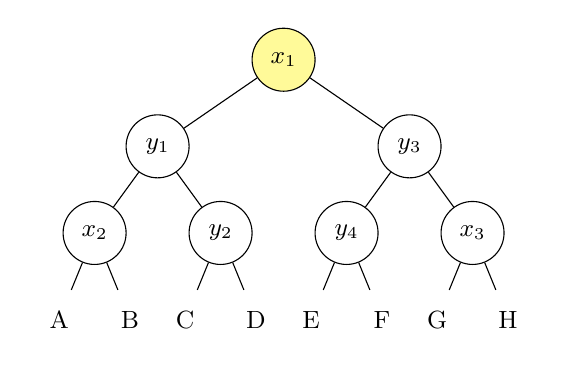
\begin{tikzpicture}[
  level distance=1.1cm,
  level 1/.style={sibling distance=3.2cm},
  level 2/.style={sibling distance=1.6cm},
  level 3/.style={sibling distance=0.9cm},
  every node/.style={circle, draw, minimum size=8mm, inner sep=1pt, font=\small},
  edge from parent/.style={draw,-}
]
\node[fill=yellow!40] {$x_1$}
  child { node {$y_1$}
    child { node {$x_2$}
      child { node[draw=none] {A} }
      child { node[draw=none] {B} }
    }
    child { node {$y_2$}
      child { node[draw=none] {C} }
      child { node[draw=none] {D} }
    }
  }
  child { node {$y_3$}
    child { node {$y_4$}
      child { node[draw=none] {E} }
      child { node[draw=none] {F} }
    }
    child { node {$x_3$}
      child { node[draw=none] {G} }
      child { node[draw=none] {H} }
    }
  };
\end{tikzpicture}
\end{minipage}%
\begin{minipage}{0.4\textwidth}
\centering
\includegraphics[width=\textwidth]{images/kdtreerange.png}
\end{minipage}
\end{center}

\textbf{Step 2: Search left child ($y_1$)}

This node splits on y. We check:
\begin{itemize}
    \item Is $y_s \leq y_1$? \textbf{No} $\rightarrow$ don't search left child
    \item Is $y_e \geq y_1$? \textbf{Yes} $\rightarrow$ search right child
\end{itemize}

The range is entirely above $y_1$, so we only search the right child. This prunes the entire lower-left region (points A and B).

\begin{center}
\begin{minipage}{0.55\textwidth}
\centering
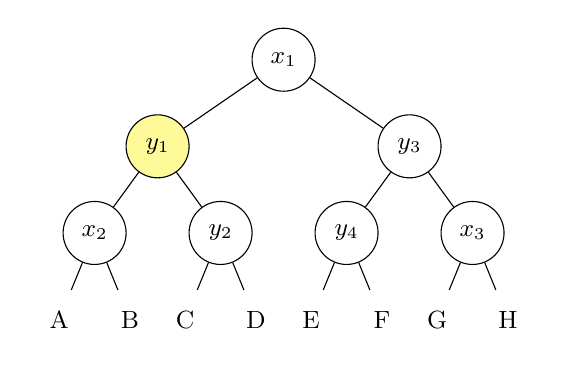
\begin{tikzpicture}[
  level distance=1.1cm,
  level 1/.style={sibling distance=3.2cm},
  level 2/.style={sibling distance=1.6cm},
  level 3/.style={sibling distance=0.9cm},
  every node/.style={circle, draw, minimum size=8mm, inner sep=1pt, font=\small},
  edge from parent/.style={draw,-}
]
\node {$x_1$}
  child { node[fill=yellow!40] {$y_1$}
    child { node {$x_2$}
      child { node[draw=none] {A} }
      child { node[draw=none] {B} }
    }
    child { node {$y_2$}
      child { node[draw=none] {C} }
      child { node[draw=none] {D} }
    }
  }
  child { node {$y_3$}
    child { node {$y_4$}
      child { node[draw=none] {E} }
      child { node[draw=none] {F} }
    }
    child { node {$x_3$}
      child { node[draw=none] {G} }
      child { node[draw=none] {H} }
    }
  };
\end{tikzpicture}
\end{minipage}%
\begin{minipage}{0.4\textwidth}
\centering
\includegraphics[width=\textwidth]{images/kdtreerange.png}
\end{minipage}
\end{center}

\textbf{Step 3: Search $y_1$'s right child ($y_2$)}

This node splits on y. We check:
\begin{itemize}
    \item Is $y_s \leq y_2$? \textbf{Yes} $\rightarrow$ search left child (point C)
    \item Is $y_e \geq y_2$? \textbf{Yes} $\rightarrow$ search right child (point D)
\end{itemize}

At leaf C, check if C is in range: \textbf{Yes!} C is \textbf{in range}.

At leaf D, check if D is in range: \textbf{Yes!} D is \textbf{in range}.

\begin{center}
\begin{minipage}{0.55\textwidth}
\centering
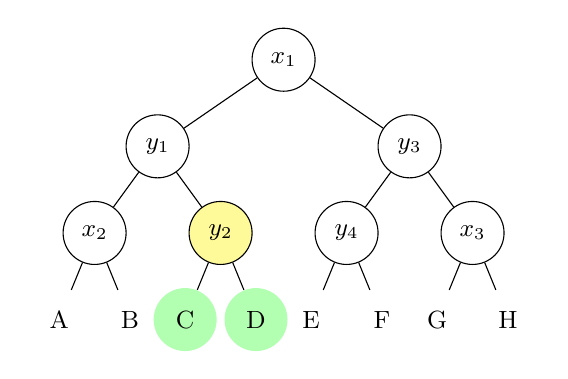
\begin{tikzpicture}[
  level distance=1.1cm,
  level 1/.style={sibling distance=3.2cm},
  level 2/.style={sibling distance=1.6cm},
  level 3/.style={sibling distance=0.9cm},
  every node/.style={circle, draw, minimum size=8mm, inner sep=1pt, font=\small},
  edge from parent/.style={draw,-}
]
\node {$x_1$}
  child { node {$y_1$}
    child { node {$x_2$}
      child { node[draw=none] {A} }
      child { node[draw=none] {B} }
    }
    child { node[fill=yellow!40] {$y_2$}
      child { node[draw=none,fill=green!30] {C} }
      child { node[draw=none,fill=green!30] {D} }
    }
  }
  child { node {$y_3$}
    child { node {$y_4$}
      child { node[draw=none] {E} }
      child { node[draw=none] {F} }
    }
    child { node {$x_3$}
      child { node[draw=none] {G} }
      child { node[draw=none] {H} }
    }
  };
\end{tikzpicture}
\end{minipage}%
\begin{minipage}{0.4\textwidth}
\centering
\includegraphics[width=\textwidth]{images/kdtreerange.png}
\end{minipage}
\end{center}

\textbf{Step 4: Back to root, search right child ($y_3$)}

Now we explore the right subtree of the root. This node splits on y. We check:
\begin{itemize}
    \item Is $y_s \leq y_3$? \textbf{No} $\rightarrow$ don't search left child
    \item Is $y_e \geq y_3$? \textbf{Yes} $\rightarrow$ search right child
\end{itemize}

The range is entirely above $y_3$, so we only search the right child. This prunes the lower-right region (points E and F).

\begin{center}
\begin{minipage}{0.55\textwidth}
\centering
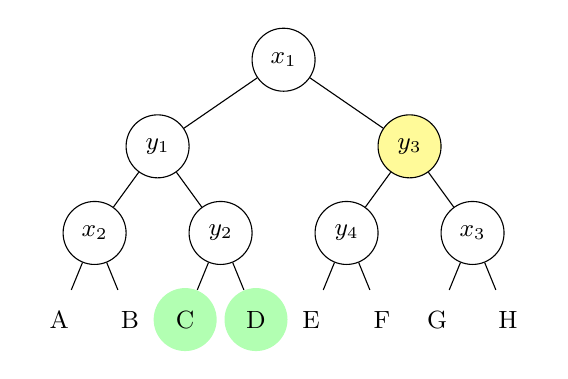
\begin{tikzpicture}[
  level distance=1.1cm,
  level 1/.style={sibling distance=3.2cm},
  level 2/.style={sibling distance=1.6cm},
  level 3/.style={sibling distance=0.9cm},
  every node/.style={circle, draw, minimum size=8mm, inner sep=1pt, font=\small},
  edge from parent/.style={draw,-}
]
\node {$x_1$}
  child { node {$y_1$}
    child { node {$x_2$}
      child { node[draw=none] {A} }
      child { node[draw=none] {B} }
    }
    child { node {$y_2$}
      child { node[draw=none,fill=green!30] {C} }
      child { node[draw=none,fill=green!30] {D} }
    }
  }
  child { node[fill=yellow!40] {$y_3$}
    child { node {$y_4$}
      child { node[draw=none] {E} }
      child { node[draw=none] {F} }
    }
    child { node {$x_3$}
      child { node[draw=none] {G} }
      child { node[draw=none] {H} }
    }
  };
\end{tikzpicture}
\end{minipage}%
\begin{minipage}{0.4\textwidth}
\centering
\includegraphics[width=\textwidth]{images/kdtreerange.png}
\end{minipage}
\end{center}

\textbf{Step 5: Search $y_3$'s right child ($x_3$)}

This node splits on x. We check:
\begin{itemize}
    \item Is $x_s \leq x_3$? \textbf{Yes} $\rightarrow$ search left child (point G)
    \item Is $x_e \geq x_3$? \textbf{No} $\rightarrow$ don't search right child
\end{itemize}

At leaf G, check if G is in range: \textbf{Yes!} G is \textbf{in range}.

We don't need to check H because the range doesn't extend past $x_3$.

\begin{center}
\begin{minipage}{0.55\textwidth}
\centering
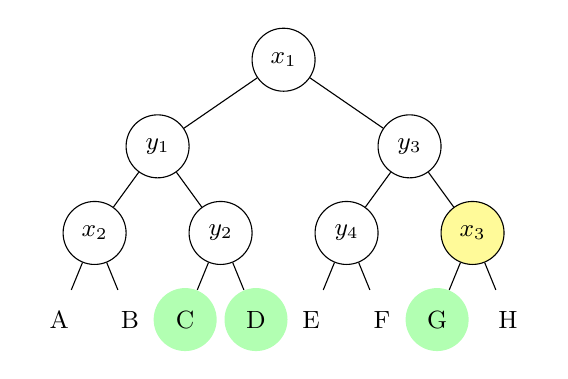
\begin{tikzpicture}[
  level distance=1.1cm,
  level 1/.style={sibling distance=3.2cm},
  level 2/.style={sibling distance=1.6cm},
  level 3/.style={sibling distance=0.9cm},
  every node/.style={circle, draw, minimum size=8mm, inner sep=1pt, font=\small},
  edge from parent/.style={draw,-}
]
\node {$x_1$}
  child { node {$y_1$}
    child { node {$x_2$}
      child { node[draw=none] {A} }
      child { node[draw=none] {B} }
    }
    child { node {$y_2$}
      child { node[draw=none,fill=green!30] {C} }
      child { node[draw=none,fill=green!30] {D} }
    }
  }
  child { node {$y_3$}
    child { node {$y_4$}
      child { node[draw=none] {E} }
      child { node[draw=none] {F} }
    }
    child { node[fill=yellow!40] {$x_3$}
      child { node[draw=none,fill=green!30] {G} }
      child { node[draw=none] {H} }
    }
  };
\end{tikzpicture}
\end{minipage}%
\begin{minipage}{0.4\textwidth}
\centering
\includegraphics[width=\textwidth]{images/kdtreerange.png}
\end{minipage}
\end{center}

\textbf{Final Result:} Points in range: \textbf{C, D, G}

\subsubsection*{Why Must We Check at the Leaf?}

Reaching a leaf does \textbf{not} guarantee the point is in range. Each split only checks \textbf{one dimension} at a time:
\begin{itemize}
    \item An x-split filters based on x only
    \item A y-split filters based on y only
\end{itemize}

We don't verify both dimensions together until we reach the leaf. For example, point B was reached because the range overlapped its region, but B's actual y-coordinate was outside $[y_s, y_e]$.

The cost of range search depends on how many branches we must explore:

\[
\text{Cost} = (\log_2(B \cdot R) + 1) \cdot (\text{number of matching pages}) \cdot D
\]

\begin{itemize}
    \item \textbf{Best case:} The range is small and falls entirely within one region at each level. We follow a single path down, similar to point lookup.
    \item \textbf{Worst case:} The range covers most of the space, and we must visit nearly all nodes (degrades to a full scan).
    \item \textbf{Typical case:} Pruning eliminates large portions of the tree. In our example, we skipped A, B, E, F, and H entirely.
\end{itemize}

The actual cost depends on how large the range is relative to the data distribution.

\subsection{Nearest Neighbor Search}

Nearest neighbor search finds the closest point to a given query point $P$. This is useful for applications like finding the nearest star to a location, or the closest monster to a game character.

\textbf{Naive approach:} Scan all points and compute the distance to each one. Cost: $B \cdot D$ (full table scan).

\textbf{Better approach:} Use the KD tree to prune regions that cannot contain a closer point.

\textbf{Algorithm:}
\begin{enumerate}
    \item Traverse down the tree as if inserting $P$, keeping track of the closest point found so far.
    \item At each leaf, check if the point is closer than the current best.
    \item \textbf{Backtrack} up the tree, checking if other branches could contain a closer point.
    \item Use geometry to prune: if the closest possible point in a region is farther than the current best, skip that entire branch.
\end{enumerate}

\textbf{Key insight:} We can avoid searching entire subtrees by computing the minimum possible distance from $P$ to any point in that region. If this minimum distance exceeds our current best, there's no point searching there.

\subsubsection*{Step-by-Step Example}

Using the KD tree from construction, suppose we want to find the nearest neighbor to point $P$ (the red square in the figure).

\textbf{Step 1: Traverse down as if inserting $P$}

Starting at the root ($x_1$), we compare $P.x$ with $x_1$. Since $P.x > x_1$, we go right to $y_3$.

At $y_3$, we compare $P.y$ with $y_3$. Since $P.y < y_3$, we go left to $y_4$.

At $y_4$, we compare $P.y$ with $y_4$. Since $P.y < y_4$, we go left to $E$.

We've reached leaf $E$. Set $E$ as our current best.

\begin{center}
\begin{minipage}{0.55\textwidth}
\centering
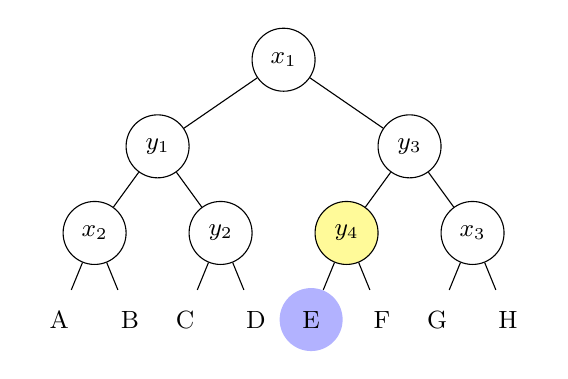
\begin{tikzpicture}[
  level distance=1.1cm,
  level 1/.style={sibling distance=3.2cm},
  level 2/.style={sibling distance=1.6cm},
  level 3/.style={sibling distance=0.9cm},
  every node/.style={circle, draw, minimum size=8mm, inner sep=1pt, font=\small},
  edge from parent/.style={draw,-}
]
\node {$x_1$}
  child { node {$y_1$}
    child { node {$x_2$}
      child { node[draw=none] {A} }
      child { node[draw=none] {B} }
    }
    child { node {$y_2$}
      child { node[draw=none] {C} }
      child { node[draw=none] {D} }
    }
  }
  child { node {$y_3$}
    child { node[fill=yellow!40] {$y_4$}
      child { node[draw=none,fill=blue!30] {E} }
      child { node[draw=none] {F} }
    }
    child { node {$x_3$}
      child { node[draw=none] {G} }
      child { node[draw=none] {H} }
    }
  };
\end{tikzpicture}
\end{minipage}%
\begin{minipage}{0.4\textwidth}
\centering
\includegraphics[width=\textwidth]{images/nearestNeighbour.png}
\end{minipage}
\end{center}

\textbf{Step 2: Backtrack to $y_4$, check sibling $F$}

We backtrack to $y_4$ and check if the other child ($F$) could contain a closer point.

The region containing $F$ is above $y_4$. We compute the minimum distance from $P$ to this region. Since $F$ is closer to $P$ than $E$, we update our best to $F$.

\begin{center}
\begin{minipage}{0.55\textwidth}
\centering
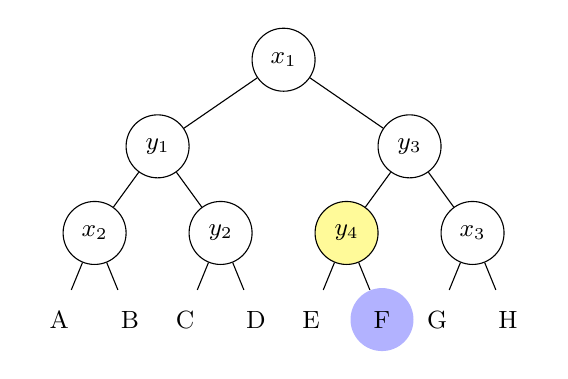
\begin{tikzpicture}[
  level distance=1.1cm,
  level 1/.style={sibling distance=3.2cm},
  level 2/.style={sibling distance=1.6cm},
  level 3/.style={sibling distance=0.9cm},
  every node/.style={circle, draw, minimum size=8mm, inner sep=1pt, font=\small},
  edge from parent/.style={draw,-}
]
\node {$x_1$}
  child { node {$y_1$}
    child { node {$x_2$}
      child { node[draw=none] {A} }
      child { node[draw=none] {B} }
    }
    child { node {$y_2$}
      child { node[draw=none] {C} }
      child { node[draw=none] {D} }
    }
  }
  child { node {$y_3$}
    child { node[fill=yellow!40] {$y_4$}
      child { node[draw=none] {E} }
      child { node[draw=none,fill=blue!30] {F} }
    }
    child { node {$x_3$}
      child { node[draw=none] {G} }
      child { node[draw=none] {H} }
    }
  };
\end{tikzpicture}
\end{minipage}%
\begin{minipage}{0.4\textwidth}
\centering
\includegraphics[width=\textwidth]{images/nearestNeighbour.png}
\end{minipage}
\end{center}

\textbf{Step 3: Backtrack to $y_3$, check sibling subtree ($x_3$)}

We backtrack to $y_3$ and check if the region above $y_3$ (containing $G$ and $H$) could have a closer point.

The minimum distance from $P$ to this upper-right region is greater than the distance from $P$ to $F$. Therefore, we \textbf{prune} this entire subtree—no need to check $G$ or $H$.

\begin{center}
\begin{minipage}{0.55\textwidth}
\centering
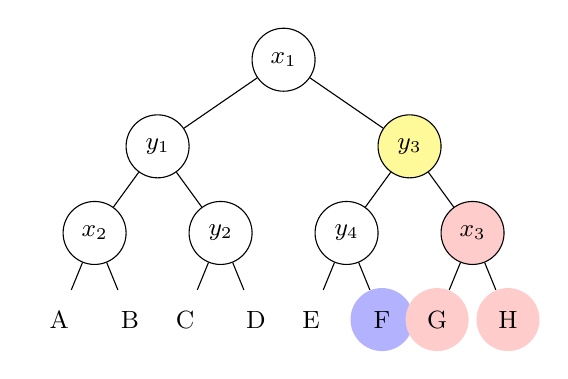
\begin{tikzpicture}[
  level distance=1.1cm,
  level 1/.style={sibling distance=3.2cm},
  level 2/.style={sibling distance=1.6cm},
  level 3/.style={sibling distance=0.9cm},
  every node/.style={circle, draw, minimum size=8mm, inner sep=1pt, font=\small},
  edge from parent/.style={draw,-}
]
\node {$x_1$}
  child { node {$y_1$}
    child { node {$x_2$}
      child { node[draw=none] {A} }
      child { node[draw=none] {B} }
    }
    child { node {$y_2$}
      child { node[draw=none] {C} }
      child { node[draw=none] {D} }
    }
  }
  child { node[fill=yellow!40] {$y_3$}
    child { node {$y_4$}
      child { node[draw=none] {E} }
      child { node[draw=none,fill=blue!30] {F} }
    }
    child { node[fill=red!20] {$x_3$}
      child { node[draw=none,fill=red!20] {G} }
      child { node[draw=none,fill=red!20] {H} }
    }
  };
\end{tikzpicture}
\end{minipage}%
\begin{minipage}{0.4\textwidth}
\centering
\includegraphics[width=\textwidth]{images/nearestNeighbour.png}
\end{minipage}
\end{center}

\textbf{Step 4: Backtrack to root, check left subtree ($y_1$)}

We backtrack to the root ($x_1$) and check if the left half of the space could contain a closer point.

We traverse down to $y_1$. The region below $y_1$ (containing $A$ and $B$) could potentially have a closer point, so we check it.

At $x_2$, we find that $B$ is closer to $P$ than $F$! Update our best to $B$.

\begin{center}
\begin{minipage}{0.55\textwidth}
\centering
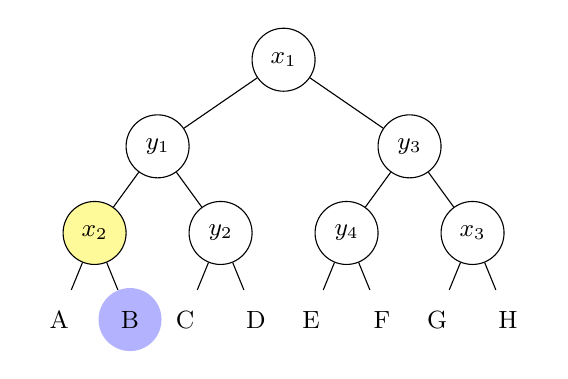
\begin{tikzpicture}[
  level distance=1.1cm,
  level 1/.style={sibling distance=3.2cm},
  level 2/.style={sibling distance=1.6cm},
  level 3/.style={sibling distance=0.9cm},
  every node/.style={circle, draw, minimum size=8mm, inner sep=1pt, font=\small},
  edge from parent/.style={draw,-}
]
\node {$x_1$}
  child { node {$y_1$}
    child { node[fill=yellow!40] {$x_2$}
      child { node[draw=none] {A} }
      child { node[draw=none,fill=blue!30] {B} }
    }
    child { node {$y_2$}
      child { node[draw=none] {C} }
      child { node[draw=none] {D} }
    }
  }
  child { node {$y_3$}
    child { node {$y_4$}
      child { node[draw=none] {E} }
      child { node[draw=none] {F} }
    }
    child { node {$x_3$}
      child { node[draw=none] {G} }
      child { node[draw=none] {H} }
    }
  };
\end{tikzpicture}
\end{minipage}%
\begin{minipage}{0.4\textwidth}
\centering
\includegraphics[width=\textwidth]{images/nearestNeighbour.png}
\end{minipage}
\end{center}

\textbf{Step 5: Check if upper-left region could have closer point}

We check if the region above $y_1$ (containing $C$ and $D$) could have a closer point than $B$.

The minimum distance from $P$ to this region is greater than the distance from $P$ to $B$. Therefore, we \textbf{prune} this subtree—no need to check $C$ or $D$.

\begin{center}
\begin{minipage}{0.55\textwidth}
\centering
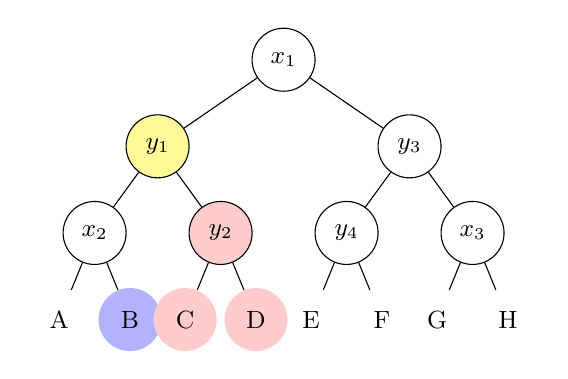
\begin{tikzpicture}[
  level distance=1.1cm,
  level 1/.style={sibling distance=3.2cm},
  level 2/.style={sibling distance=1.6cm},
  level 3/.style={sibling distance=0.9cm},
  every node/.style={circle, draw, minimum size=8mm, inner sep=1pt, font=\small},
  edge from parent/.style={draw,-}
]
\node {$x_1$}
  child { node[fill=yellow!40] {$y_1$}
    child { node {$x_2$}
      child { node[draw=none] {A} }
      child { node[draw=none,fill=blue!30] {B} }
    }
    child { node[fill=red!20] {$y_2$}
      child { node[draw=none,fill=red!20] {C} }
      child { node[draw=none,fill=red!20] {D} }
    }
  }
  child { node {$y_3$}
    child { node {$y_4$}
      child { node[draw=none] {E} }
      child { node[draw=none] {F} }
    }
    child { node {$x_3$}
      child { node[draw=none] {G} }
      child { node[draw=none] {H} }
    }
  };
\end{tikzpicture}
\end{minipage}%
\begin{minipage}{0.4\textwidth}
\centering
\includegraphics[width=\textwidth]{images/nearestNeighbour.png}
\end{minipage}
\end{center}

\textbf{Final Result:} Nearest neighbor to $P$ is \textbf{B}.

\subsubsection*{How Pruning Works}

To decide whether to search a region, we compute the \textbf{minimum possible distance} from $P$ to any point in that region:

\begin{itemize}
    \item For a region defined by split lines, find the closest point on the region's boundary to $P$.
    \item If this minimum distance is greater than the distance to our current best, skip the entire region.
\end{itemize}

In geometric terms, imagine drawing a circle around $P$ with radius equal to the distance to the current best. If a region doesn't intersect this circle, it cannot contain a closer point.

\subsubsection*{Key Observations}

\begin{itemize}
    \item \textbf{Pruning saves work:} We skipped $G$, $H$, $C$, and $D$ entirely because their regions couldn't contain a closer point.
    \item \textbf{Order matters:} The initial traversal path affects how quickly we find a good candidate. A closer initial guess leads to more pruning.
    \item \textbf{Must backtrack:} Unlike range search, we can't just follow one path. The nearest neighbor might be in a different branch than where $P$ would be inserted.
    \item \textbf{Worst case:} If points are distributed poorly, we may need to visit many nodes. But typically, pruning eliminates large portions of the tree.
\end{itemize}

\subsubsection*{I/O Cost}

The cost depends on how much pruning occurs:

\begin{itemize}
    \item \textbf{Best case:} The nearest neighbor is found on the initial traversal, and all other branches are pruned. Cost: $(\log_2(B \cdot R) + 2) \cdot D$ (same as point lookup).
    \item \textbf{Worst case:} Little pruning occurs, and we visit most nodes. Cost approaches $B \cdot D$ (full scan).
    \item \textbf{Typical case:} Pruning eliminates most branches. Cost is a small multiple of $\log_2(B \cdot R)$.
\end{itemize}

\subsection{Insertion and Deletion}

To insert a new point, traverse to find where it belongs, then add it.

\[
\text{Cost} = (\log_2(B \cdot R) + 4) \cdot D
\]

\begin{itemize}
    \item $\log_2(B \cdot R) + 1$: traverse down the tree (the $+1$ adjusts for the fact that $\log_2(n)$ gives levels minus one)
    \item $+3$: read the data page, write the data page, and write a new index node
\end{itemize}

To delete a point, find it first, then remove it.

\[
\text{Cost} = (\log_2(B \cdot R) + 4) \cdot D
\]

\begin{itemize}
    \item $\log_2(B \cdot R) + 1$: traverse down the tree
    \item $+3$: read the data page, write the modified data page, and potentially update an index node
\end{itemize}

Unlike B+ trees, KD trees do not have splitting or merging operations to maintain balance. Repeated insertions and deletions can cause the tree to become unbalanced, leading to deeper traversals and worse query performance. This is why databases typically \textbf{bulk load} KD trees.

\subsection{I/O Cost Summary}

\begin{table}[H]
    \centering
    \begin{tabular}{lc}
        \toprule
        \textbf{Operation} & \textbf{KD Tree} \\
        \midrule
        Scan all records & $B \cdot D$ \\
        Point Lookup & $(\log_2(B \cdot R) + 2) \cdot D$ \\
        Range Search & $(\log_2(B \cdot R) + 1) \cdot \text{pages} \cdot D$ \\
        Insert & $(\log_2(B \cdot R) + 4) \cdot D$ \\
        Delete & $(\log_2(B \cdot R) + 4) \cdot D$ \\
        \bottomrule
    \end{tabular}
    \caption{KD Tree I/O cost (in page reads)}
\end{table}

\end{document}